\documentclass{article}

\usepackage{amsmath}
\usepackage{amssymb}
\usepackage{mathtools}
\usepackage{fullpage}
\usepackage{enumerate}
\usepackage{graphicx}

\title{Computer Science 760 Notes \\ Machine Learning}
\author{Mendel C. Mayr}
\date{\today}

\begin{document}
	\maketitle
	\vspace{10pt}
	\begin{center}
		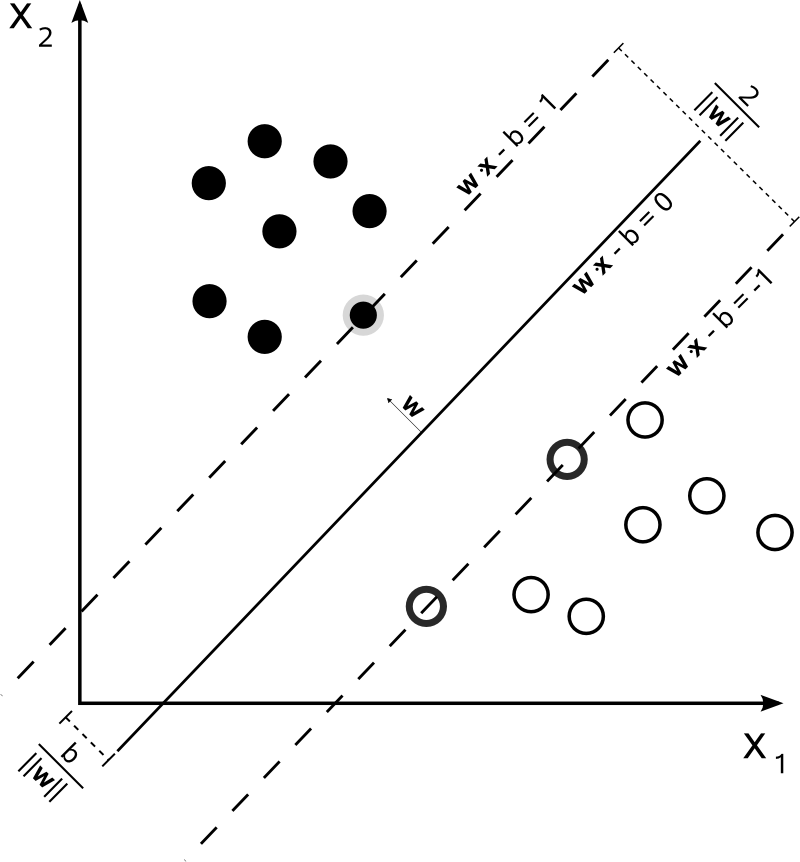
\includegraphics[width = 2.9in]{svm.png}
		\end{center}
	\vspace{16pt}
	\tableofcontents
	\clearpage

	\section{Decision Tree Learning}
		\subsection{Information Gain}
			Information gain is used to determine the (feature to) split \\
			Information theory: entropy and information gain:
			\begin{enumerate}[(i)]
				\item Entropy $= H(X) = -\sum_{x \in X}P(X = x)\log_2 P(X = x)$
				\item Conditional entropy $= H(Y|X) = -\sum_{x \in X}P(Y|X = x)$, where \\
				$H(Y|X = x) = \sum_{y \ in Y}P(Y = y|X = x)\log_2 P(Y = y|X = x)$
				\item Mutual information (information gain) $= I(X, Y) = H(Y) - H(Y|X)$
				\end{enumerate}
			Alternative metric: Gini coefficient, i.e. product of probabilities for each of (2) outcomes for the feature \\
			\\
			Limitation of information gain: biased toward tests with many outcomes (i.e. features with many possible values) \\
			C4.5 uses gain ratio: $SplitInfo(D, S) = -\sum_{k \in S} |D_k|/|D| \log_2(D_k/D)$, and $GainRatio = I(D, S)/SplitInfo(D, S)$
		\subsection{Decision Tree Algorithms}
			Overfitting: $h \in H$ overfits the training data $D$ if there is an alternative model $h' \in H$ such that $error(h) > error(h')$ yet $error_D(h) < error_D(h)$ \\
			Avoiding overfitting in decision tree learning:
			\begin{enumerate}[(i)]
				\item Early stopping: stop if further splitting not justified by statistical test
				\item Post-pruning: grow large tree, then prune nodes using tuning set \\
				Iteratively eliminate nodes until further reductions reduce accuracy
				\end{enumerate}
			Lookahead: instead of evaluating using information gain, look ahead to see what splits at the next level would be, and measure information gain at a deeper level \\
			\\
			Continuous features: use threshold-based boolean attribute, treshold determined by sorting examples according to the featurem and generating candidate thresholds between adjacent examples with different class values \\
			Threshold chosen from candidates based on information gain \\
			\\
			Training examples with missing attribute values: possible strategies
			\begin{enumerate}[(i)]
				\item At node $n$, upon encountering a missing feature value, assign it the value most common among examples at node $n$, or most common among examples at the node $n$ that also have the same class value
				\item Assign fractional value to attribute for the example and pass fractional example to children for purposes of evaluating information gain
				\end{enumerate}
		\clearpage

	\section{Instance-Based Learning}
		\subsection{K-nearest Neighbor}
			$k$-nearest neighbor classification: given an instance $x_q$ to classify, find $k$ training-set instances that are most simimlar or $x_q$ \\
			Return the class value: $\hat{y} = argmax_{v \in values(Y)} \sum_{i = 1}^k \delta(v, y_i)$ \\
			Various determinations of distance: 
			\begin{enumerate}[(i)]
				\item Hamming distance: number of features with differing values
				\item Euclidean distance: $\delta(x_i, x_j) = \sqrt{\sum_f ({x_i}_f - {x_j}_f)^2}$
				\item Manhattan distance: $\delta(x_i, x_j) = \sum_f ({x_i}_f - {x_j}_f)^2$
				\end{enumerate}
			$k$-nearest neighbor regression: given an instance $x_q$, find the $k$ nearest training-set instances and return $\sum_{i = 1}^k \delta(v, y_i)$ \\
			Distance-weighted nearest neighbor: instances contribute to prediction according to their distance from $x_q$ \\
			\\
			$k$-nearest neighbor does almost nothing at training time, and offsets costs to classification/prediction time \\
			Strategies to speed up $k$-nearest neighbor
			\begin{enumerate}[(i)]
				\item Don't retain every training instance: edited nearest neighbor \\
				Select subset of instances that still provide accurate classifications: \\
				\begin{enumerate}[(a)]
					\item Incremental deletion: delete from memory all training instances redundant to classification
					\item Incremental growth: if training instances insufficient to classify training instance, add to memory
					\end{enumerate}
				\item Use data structure to look up nearest neighbors ($k$-$d$ tree)
				\end{enumerate}
			$k$-$d$ trees ($A^*$ instance search): each node stores one instance, and splits on the median value of the feature having the highest variance \\
			Nodes are pushed to the $A^*$ priority queue with the value indicating the minimum possible distance to the query based on the threshold for the split \\
			\\
			Strenghts of instance based learning: simple, efficeint training, easily adapts to on-line nearning, rubust to noisy data, etc. \\
			Limitations: sensitive to range of feature values, senstivie to irrelevant and correlated features, inefficient classification, no insight into problem domain (i.e. lacks modeling of problem)
		\subsection{Linear Locally Weighted Regression}
			Locally weighted linear regression: $f(x) = w_0 + w_1a_1(x) +\:...\:+ w_na_n(x)$ \\
			Local approximations to have query point fit local training examples:
			\begin{enumerate}
				\item Minimize squared error over just $k$ nearest neighbors: \\
				$E_1(x_q) = (1/2)\sum_{x \in k\text{ nearest neighbors of }x_q} (f(x) - \hat{f}(x))^2$
				\item Minimize squared error over entire set of $D$ of training examples, using decreasing function $K$: \\
				$E_2(x_q) = (1/2)\sum_{x \in D} (f(x) - \hat{f}(x))^2 K(d(x_q, x))$
				\item Combination of the previous: let $N$ be $k$ nearest neighbors of $x_q$
				\begin{equation*}
					\frac{1}{2}\sum_{x \in N} (f(x) - \hat{f}(x))^2 K(d(x_q, x))
					\end{equation*}
				\end{enumerate}
		\clearpage

	\section{Probability and Bayesian Learning}
		Note: for more rigourous details, see Heckerman's Bayesian Network Learning Tutorial
		\subsection{Probabilistic Machine Learning Concepts}
			Recall Bayes theorem: $P(A|B) = P(B|A)P(A)/P(B)$ \\
			\\
			Brute-force MAP learning algorithm:
			\begin{enumerate}[(i)]
				\item Given information $D$, for each hypothesis $h \in H$, calculate the posterior probability $P(h|D) = P(D|h)P(h)/P(D)$
				\item Output hypothesis $h_{MAP}$ with highest posterior probability $h_{MAP} = argmax_{h \in H} P(h|D)$
				\end{enumerate}
			Other probabalisitic concepts in machine learning:
			\begin{enumerate}[(i)]
				\item Maximum likelihood and least-squared error hypotheses
				\item Maximum likelihood hypotheses for predicting probabilities
				\item Minimum description length principle
				\item Bayes optimal classification: $argmax_{v_j \in V}\sum_{h_i \in H} P(v_j|h_i)P(h_i|D)$
				\item Gibb's Algorithm: choose hypothesis $h \in H$ at random, according to posterior probaiblity distribution over $H$, and use $h$ to predict the classification of the next instance $x$ 
				\end{enumerate}
		\subsection{Bayesian networks}
			A Bayesian network consists of a directed acyclic graph and a set of conditional probability distributions \\
			In the each Directed Acyclic Graph (DAG):
			\begin{enumerate}[(i)]
				\item Each node denotes a random variable
				\item An edge from $X$ to $Y$ represents that $X$ directly influences $Y$
				\item Each node $X$ contains a conditional probability distribution representing $P(X|Parents(X))$
				\item Each variable $X$ is independent of its non-descendants given its parents
				\item Each variable $X$ is independent of all others given its Markov blanket
				\end{enumerate}
			Advantages of Bayesian network representation:
			\begin{enumerate}[(i)]
				\item Captures indepdendence and conditional indpendence where they exist
				\item Encodes the relevant  portion fo the full joint distribution
				\item Graphical representation gives insight into complexity of inference
				\end{enumerate}
			Inference task: given values for some variables in the network (evidence) and set of query variables, compute posterior distribution over query variables \\
			Hidden variables: neither evidence nor the query variables \\
			Baysean networks allow for any set to be evidence and any set to be query \\
			Inference by enumeration: consider the chain rule $P(x_1, ..., x_n) = P(x_1)P(x_2|x_1)P(x_3|x_2, x_1)...P(x_n|x_{n-1}, ..., x_1)$ \\
			Posterior probability on query variables can be found via independence, chain rule, and marginalization \\
			\\
			Parameter learning task: given set of training instances and graph structure, infer parameter of conditional probability distributions \\
			Strcture learning task: given set of training instances, infer graph structure (and possibly parameters of CPDs) \\
			For parameter learning, use maximum a posteriori (MAP) estimation: e.g. m-estimates $P(X = x) = (n_x + p_xm)/(\sum_{v \in Values(X)} n_v) + m$, where $p_x$ is prior probability of value $x$, $m$ is number of virtual instances, and $n_v$ is number of occurences of value $v$ 
		\subsection{Expectation Maximization}
			Missing data (hidden variables, values missing at random): values can be imputed using Expectation Maximization (EM) \\
			Iterate until convergence:
			\begin{enumerate}[(i)]
				\item Expectation step: using current model, compute expectation over missing values (missing temporarily take expected values)
				\item Maximization step: update model parameters with those that maximize probability of data (MLE or MAP)
				\end{enumerate}
			Note that $k$-means unsupervised clustering is a form of expectation maximization \\
			Expectation maximation can be hard (takes most likely value) or soft (expectation is probabiltiy distribution) \\
			\\
			Expectation maximation for parameter learning:
			\begin{enumerate}[(i)]
				\item Expecation step: compute probability of each completion of incomplete data points, i.e. answering query over missing variables given others
				\item Maximization step: use completed data set to update Dirchlet distributions, except counts can be fractional, update conditional probability tables
				\end{enumerate}
			Subtelty for parameter learning: overcounting based on number of iterations required to converge to settings for missing values. After each expectation step, reset Dirichlet distributions before repeating maximization step \\
			\\
			Problems with expectation maximization: only finds local optimum, deterministic with respect to priors
		\subsection{Learning Network Structure}
			Chow-Liu algorithm: learns tree structure that maximizes likelihood of training data
			\begin{enumerate}[(i)]
				\item Compute weight $I(X_i, X_j)$ of each possible edge $(X_i, X_j)$
				\item Find maximum-weight spanning tree: use mutual information to calculate \\
				$I(X, Y) = \sum_{x \in values{X}}\sum_{y \in values{Y}} P(x, y)\log_2 P(x, y)/(P(X)P(Y))$ \\
				\\
				Prim's algorithm (given $(V, E)$):
				\begin{enumerate}[(a)]
					\item $V_{new} = \{v\}$ where $v \in V$ (arbitrary)
					\item $E_{new} = \{\}$
					\item Repeat until $V_{new} = V$: choose edge $(u, v)$ in $E$ with max weight where $u$ is in $V_{new}$ and $v$ is not. Add $v$ to $V_{new}$ and $(u, v)$ to $E_{new}$
					\item Return $(V_{new}, E_{new}$, a maximum spanning tree
					\end{enumerate}
				Kruskal's algorithm (given $(V, E)$):
				\begin{enumerate}[(i)]
					\item $E_{new} = \{\}$
					\item For each $(u, v)$ in $E$ ordered by weight (high to low): \\
					Pop $(u, v)$ from $E$ and add to $E_{new}$ if it does not create a cycle
					\item Return $V$ and $E_{new}$, a maximum spanning tree
					\end{enumerate}
				\item Assign edge directions in maximimum-weight spanning tree \\
				Pick a node for the root, assign edge direction
				\end{enumerate}
			Heuristic search for structure learning: each state in search space represents Bayes net structure \\
			Search approach requires specification of
			\begin{enumerate}[(i)]
				\item Scoring function: $score(G, D) = \sum_i score(X_i, Parents(X_i):D)$ \\
				Thus, a network can be scored by summing terms over nodes, and changes can be efficently scored via a local search
				\item State transition operators: adding an edge, deleting in edge, reversing an edge
				\item Search algorithm: hill climbing or sparse candidate search
				\end{enumerate}
			Bayesian network hill climibing search: greedy algorithm \\
			Bayesian network sparse candidate search (given data set $D$, initial network $B_0$, parameter $k$):
			\begin{enumerate}[(i)]
				\item Let $i = 0$
				\item Repeat until convergence:
				\begin{enumerate}[(a)]
					\item Increment $i$
					\item Restrict step: select for each variable $X_j$ a set $C_j^i(|C_k^i|)$ of candidate parents
					\item Maximize step: find network $B_i$ maximizing score among networks where $\forall X_j, Parents(X_j) \subset C_j^i$
					\end{enumerate}
				\item Return $B_i$
				\end{enumerate}
			Restriction step in sparse candidate search: \\
			Fpr the first iteration: candidate parents computed using mutual information \\
			$I(X, Y) = \sum_{x, y} P(x, y)\log{(P(x, y)/(P(x)P(y)))}$ \\
			Kullback-Liebler divergence: distance measure between two distributions $P$ and $Q$
			\begin{equation*}
				D_{KL} = (P(X)||Q(X)) = \sum\limits_x P(x)\log\frac{P(x)}{Q(x)}
				\end{equation*}
			KL-divergence assesses discrepancy between network's estimate $P_{net}(X, Y)$ and empirical estimate \\
			$M(X, Y) = D_{KL}(P(X, Y)||P_{net}(X, Y))$ \\
			\\
			Algorithm for restriction step in sparse candidate (given data $D$, current network $B_i$, parameter $k$):
			\begin{enumerate}[(i)]
				\item For each variable $X_j$
				\begin{enumerate}[(a)]
					\item Calculate $M(X_j, X_i)$ for all $X_j \neq X_i$ such that $X_l \notin Parents(X_j)$
					\item Choose highest ranking $X_l...X_{k - s}$ where $s = |Parents(X_j)|$
					\item Include current parents in candidate set to ensure monotonic score improvements \\
					$C_j^i = Parents(X_j) \cup X_l ... X_{k - s}$
					\end{enumerate}
				\item Return ${C_j^i}$ for all $X_j$
				\end{enumerate}
			Scoring function for structure learning: maxmize data probability, but penalize complexity \\
			General approach: $argmax_{G, \theta_G} \log{P(D|G, \theta_G)} - f(n)|\theta_G|$ \\
			Akaike information criterion (AIC) $f(n) = 1$, Bayesian Information Criterion (BIC) $f(n) = \log{(n)}/2$
		\subsection{Naive Bayes and Tree Augmented Network}
			Naive Bayes assumption: all features $X_i$ are conditionally independent given class $Y$ \\
			$P(X_1, ..., X_n, Y) = P(Y)\Pi_{i = 1}^nP(X_i|Y)$ \\
			Unaugmented tree starts with edge from node $Y$ to each feature $X_1, ..., X_n$
			\\
			Learning: estimate $P(Y = y)$ for each value of $Y$, estimate $P(X_i = x|Y = y)$ for each $X_i$ \\
			Classification done using Bayes rule: 
			\begin{equation*}
				P(Y = y|X) = \frac{P(y)P(X|y)}{\sum\limits_{y' \in values(Y)}P(y')P(X|y')} = \frac{P(y)\prod\limits_{i = 1}^n P(x_i|y)}{\sum\limits_{y' = values(Y)}(P(y')\prod\limits_{i = 1}^n P(x_i|y'))}
				\end{equation*}
			Tree Augmented Network (TAN) algorithm: learns tree structure to augment edges of naive Bayes network
			\begin{enumerate}[(i)]
				\item Compute weight $I(X_i, X_j|Y)$ for each possible edge $(X_i, X_j)$ between features
				\item Find maximum weight spanning tree (MST) for graph over $X_l ... X_n$
				\item Assign edge direction in MST
				\item Construct a TAN model by adding node for $Y$ and an edge for $Y$ to each $X_i$
				\end{enumerate}
		\clearpage

	\section{Machine Learning Methdology}
		\subsection{Partitioning of Data}
			Evaluation of learning models: given instance set $X$ and probability distribution $D$ defining the probaiblity of encountering an $x \in X$, learner must learn target concept (function) $f \in H$ \\
			Evaluation methdology seeks to answer two questions: what is the best accuracy for a hypothesis $h$, learned from $n$ instances, applied to future instances drawn according to $D$, and what is the probably error in this accuracy estimate \\
			\\
			Distinction between sample error and true error:
			\begin{enumerate}[(i)]
				\item Sample error: error of $h$ with respect ot target function $f$ and data sample $S$ \\	
				$error_S(h) = (1/n)\sum_{x \in S} \delta(f(x), h(x))$, where $\delta(a, b) = 1$ if $a \neq b$, 0 otherwise
				\item True error: $error_D(h) = Pr_{x \in D} [f(x) \neq h(x)]$
				\end{enumerate}
			Limitations of singular training/test partitions: 
			\begin{enumerate}[(i)]
				\item Not enough data for sufficiently large training and test sets 
				\item Single training set does not show how sensitive accuracy is to particular training sample
				\end{enumerate}
			Random resampling: repeatedly partitioning data into training and test sets \\
			Stratified sampling: statify instances by class and select (i.e. maintain class proportions) \\
			Cross validation: partition data into $n$ subsamples. Iteratively test on one subset, train on rest \\
			Leave-one-out cross validation: $n$ is the number of instances 
		\subsection{Performance Evaluation}
			Receiver Operating Characteristic (ROC) curve: true positive-rate vs false positive-rate as threshold as confidence of an instance being positive is varied \\
			Algorithm for creating an ROC curve: 
			\begin{enumerate}[(i)]
				\item Sort test-set prediction according to confidence that each instance is positive
				\item Step through sorted list from high to low confidence
				\begin{enumerate}[(a)]
					\item Locate threshold between instances with opposite classes
					\item Compute TPR, FPR for instances above threshold
					\item Output (FPR, TPR) coordinate
					\end{enumerate}
				\end{enumerate}
			Points plotted on ROC curve can be interpolated to form convex hull \\
			Having a high TPR or low FPR does not indicate accuracy in unbalanced data sets \\
			\\
			Alternative accuracy metric: recall and precision
			\begin{enumerate}[(i)]
			 	\item Recall (TP rate) = TP/(actual positives) = TP/(TP + FN)
			 	\item Precision = TP/(predicted positives) = TP/(TP + FP)
				\end{enumerate}
			Precision/recall curve: plots prevision vs. recall as threshold as confidence of an instance being positive is varied \\
			\\
			Single ROC/PR curve with cross-validation: multiple approaches
			\begin{enumerate}[(i)]
				\item Assume confidence values comparable across folds \\
				Pool predicitons from all test sets and plot curve from pooled predictions
				\item Plot individual curves for all test sets, viewing each as function \\
				Plot average curve for set of functions 
				\end{enumerate}
			ROC and PR curves allow predictive performance to be assessed at various levels of confidence, assume binary classification, and can be summarized by the integral \\
			ROC curves: insensitive to class distribution changes, can identify optimal classification thresholds for tasks with differential misclassification costs \\
			PR curves: show fraction of predictions that are false positives, suited for tasks with many negative instances
		\subsection{Confidence Intervals and Learning Tasks}
			Avoiding pitfalls: questions when applying learning tasks
			\begin{enumerate}[(i)]
				\item Held-aside test data should be representative of collecting new data
				\item Folds of cross validation should only use training data for the fold \\
				At no point in preprocessing should test case labels be accessed
				\item Repeated modificiations of learning algorithm or preprocessing could lead to overfitting
				\end{enumerate}
			Confidence intervals on error: suppose we have learned model $h$, test set $S$ containing $n$ instances drawn independently of each other and independent of $h$, with $n \geq 30$, and $h$ makes $r$ errors over the $n$ instances \\
			Estimate of error is $error_S(h) = r/n$ \\
			With approximately $N$ probability, the true error is in the interval
			\begin{equation*}
				error_S(h) \pm z_N \sqrt{\frac{error_S(h)(1 - error_S(h))}{n}}
				\end{equation*}
			where $z_N$ is a constant that depends on $N$, e.g. $z_{0.95} = 1.96$ \\
			Confidence interval follows from normal approximation of binomial distribution \\
			An $N\%$ confidence interval on parameter $p$ is an interal that is expected with $N\%$ probability to contain $p$ \\
			In using confidence intervals, consider (central limit theorem) that a large number independent, identically distribution random variables approximately follows a normal distribution \\
			\\
			Difference in error of two hypotheses: $\hat{d} = error_S(h_1) - error_S(h_2)$ \\
			$N\%$ confidence interval for $d$ is:
			\begin{equation*}
			 	\hat{d} \pm z_N \sqrt{\frac{error_{S_1}(h_1)(1 - error_{S_1}(h_1))}{n_1} + \frac{error_{S_2}(h_2)(1 - error_{S_2}(h_2))}{n_2}}
				\end{equation*}
		\subsection{Comparing Learning Models and Hypotheses}
			Consider $\delta$s as observed values of a set of independent, identically distributed variables \\
			Null hypothesis: the 2 learning systems have the same accuracy \\
			Alternative hypothesis: one system is more accurate than the other \\
			Hypothesis test:
			\begin{enumerate}[(i)]
				\item Use paired $t$-test to determine probability $p$ that mean of $\delta$s would arise from null hypothesis
				\item If $p$ is sufficiently small (usually $p < 0.05$), reject null hypothesis
				\end{enumerate}
			Comparing systems using a paired $t$-test: 
			\begin{enumerate}[(i)]
				\item Calculate sample mean: $\bar{\delta} = (1/n)\sum_{i = 1}^n \delta_i$
				\item Calculate $t$ statistic:
				\begin{equation*}
					t = \frac{\bar{\delta}}{\sqrt{\frac{1}{n(n - 1)}\sum\limits_{i = 1}^n (\delta_i - \bar{\delta})^2}}
					\end{equation*}
				\item Determine corresponding $p$-value: use $t$ in table for $t$-distribution with $n - l$ degrees of freedom
				\end{enumerate}
			$t$-tests compare two learning systems, tests like McNemar's $\chi^2$ test compares two learned models \\
			\\
			Scatter plots for pairwise method comparison: can compare thwo methods $A$ and $B$ by plotting $(A perf., B perf.)$ across numerous data sets \\
			Lesion studies: determine relevant contributions to learning system performance by removing (lesioning) components
		\clearpage

	\section{Computational Learning Theory}
		\subsection{PAC Learning}
			Computational learning theory concerns itself with: 
			\begin{enumerate}[(i)]
				\item Sample complexity: how many training examples needed to converge on hypothesis
				\item Computational complexity: how much computational effort needed for learner to converge
				\item Mistake bound: how many misclassifications before learner converges on hypothesis
				\end{enumerate}
			Learning setting composed of:
			\begin{enumerate}[(i)]
				\item Set of instances $X$
				\item Set of hypotheses $H$
				\item Set of possible target concepts $C$
				\item Unknown probability distribution $D$ over instances
				\end{enumerate}
			Learner is given set $D$ of training instances $(x, c(x))$ for some target concept $c \in C$ \\
			Learning task is to output hypothesis $h$ modeling $c$ \\
			\\
			True error of hypothesis: how often $h$ is wrong on future instances drawn from $D$: \\
			$error_D(h) = P_{x \in D}(c(x) \neq h(x))$ \\
			Traning error: how often $h$ is wrong on instances in training set $d$ \\
			$error_D(h) = P(x \in D)(c(x) \neq h(x)) = (1/|D|)\sum_{x \in D}\delta(c(x) \neq h(x))$ \\
			\\
			Probably Approximately Correct (PAC) Learning: consider class $C$ of possible target concepts defined over set of instances $X$ each of length $n$, and a learner $L$ using hypothesis space $H$ \\
			\\
			Formal definition of PAC Learnable: \\
			$C$ is PAC learnable by $L$ if for all $c \in C$, distributions $D$ over $C$, $\varepsilon$ and $\delta$ such that $0 < \varepsilon, \delta < 0.5$ : \\
			Learner $L$ will, with probability greater than $(1 - \delta)$, output hypothesis $h \in H$ such that $error_D(h) \leq \varepsilon$, in time polynomial to $1/\varepsilon, 1/\delta, n, size(c)$ \\
			\\
			Suppose hypotheses consistent with $m$ training instances \\
			PAC learnability determined by whether:
			\begin{enumerate}[(i)]
				\item $m$ grows polynomially in the relevant parameters
				\item Processing time per training example is polynomial
				\end{enumerate}
			Consistency with respect to training example set $D = \{(x_1, c(x_1), ..., (x_m, c(x_m)))\}$, and hypothesis $h$
			\begin{equation*}
				consistent(h, D) = \forall((x, c(x)) \in D) h(x) = c(x)
				\end{equation*}
			Version space: $VS_{H, D} = \{h \in H | consistent(h, D)\}$ \\
			Version space $VS_{H, D}$ is $\varepsilon$-exhausted with repsect to concept $c$ and data set $D$ if: \\
			$(\forall h \in VS_{H, D}) error_D(h) < \varepsilon$ \\
			\\
			The probability that $VS_{HD}$ is not $\varepsilon$-exhausted is no greater than $|H|e^{-\varepsilon m}$ \\
			Proof: probability that some hypothesis with error greater than $\varepsilon$ is consistent with $m$ training instance is $(1 - \varepsilon)^m$, there are at most $|H|$ such hypotheses, and since $(1 - \varepsilon) \geq e^{-\varepsilon}$ when $0 \leq \varepsilon \leq 1$, the bound is $|H|e^{-\varepsilon m}$ \\
			\\
			The probability must be reduced below $\delta$: $|H|e^{-\varepsilon m} \geq \delta$ \\
			Solving for $m$ yields the number of examples needed for PAC learnability:
			\begin{equation*}
				m \geq \frac{1}{\varepsilon}\left(\ln{|H|} + \ln{\frac{1}{\delta}}\right)
				\end{equation*}
		\subsection{Hypothesis Spaces}
			Agnostic learning setting: don't assume $c \in H$ \\
			Learner returns hypothesis $h$ that makes fewest errors in training \\
			For training set error to be less than $error_D(h) + \varepsilon$, $m$ examples sufficient, where
			\begin{equation*}
				m \geq \frac{1}{2\varepsilon^2}\left(\ln{|H|} + \ln{\frac{1}{\delta}}\right)
				\end{equation*}
			If $H$ is infinite, for measure of hypothesis space complexity, use in place of $|H|$ the largest subset of $X$ for which $H$ can guarantee zero training error regardless of target function \\
			\\
			A set of instances $D$ is shattered by a hypothesis space $H$ if and only if for every dichotomy of $D$, there is a hypothesis in $H$ consistent with the dichotomy \\
			The VC dimension of $H$ defined over instance space $X$ is the size of the largest finite subset of $X$ that is shattered by $H$ \\
			\\
			A concept class is PAC learnable if it has finite VC dimension \\
			The VC dimension for finite $H$: $VC-dim(H) \leq \log_2|H|$ \\
			Proof: suppose $VC-dim(H) = d$, and for $d$ instances
			\begin{enumerate}[(i)]
				\item There are at most $2^d$ different possible labelings
				\item $H$ must represent at most $2^d$ hypotheses, so $2^d \leq |H|$
				\item Thus $d \leq \log_2|H|$, so $VC-dim(H) \leq \log_2|H|$
				\end{enumerate} 
			Using $VC-dim(H)$ as a measure of complexity of $H$, the bound can be defined as
			\begin{equation*}
				m \geq \frac{1}{\varepsilon}\left(4\log_2\frac{2}{\delta} + 8VC-dim(H)\log_2\frac{13}{\varepsilon}\right)
				\end{equation*}
			Lower bound on sample complexity: given target concept $C$
			\begin{equation*}
				m < max\left[\frac{1}{\varepsilon}\log{|\frac{1}{\delta}|}, \frac{VC-dim(C) - 1}{32\varepsilon}\right]
				\end{equation*}
		\subsection{Mistake Bound}
			Learning setting (i.e. on-line learning setting): for $t = 1, 2, ...$
			\begin{enumerate}[(i)]
				\item Learner receives instance $x_t$
				\item Learner predicts $h(x_t)$
				\item Learner receives label $c(x_t)$ and updates model $h$
				\end{enumerate}
			Mistake bound model addresses how many mistakes will be made before the target concept is learned \\
			\\
			Mistake bound model analysis of halving algorithm \\
			Halving algorithm is as follows:
			\begin{enumerate}[(i)]
				\item $VS_1 = H$
				\item For $t = 1$ to $T$:
				\begin{enumerate}[(a)]
					\item Given training instance $(x_t, c(x_t))$, $h'(x_t) = MajorityVote(VS_t, x_t)$
					\item Eliminate all wrong $h$ from version space (at least half) \\
					$VS_{t + 1} = \{h \in VS_t | h(x_t) = c(x_t)\}$
					\end{enumerate}
				\item Return $VS_{t + 1}$
				\end{enumerate}
			Maximum number of mistakes is $M_{Halving}(C) = \lfloor\log_2|H|\rfloor$ \\
			\\
			Optimal mistake bounds: suppose $C$ is an arbitrary nonempty concept class \\
			An optimal mistake bound is defined as $Opt(C) = min_{A \in \text{Learning Algorithms}} M_A(C)$ \\
			$M_{Opt}(C)$ is defined as the number of mistakes made given:
			\begin{enumerate}
			 	\item The hardest target concept to learn
			 	\item The hardest training sequence and distribution
			 	\item Using the best algorithm to determine the concept
				\end{enumerate} 
			Optimal mistake bound is $VC-dim(C) \leq M_{Opt}(C) \leq M_{Halving}(C) \leq log_2(|C|)$ \\
			In short $M_{Opt}(C) \geq VC-dim(C)$, the mistake bound is no lower than the concept's VC-dimension \\
			\\
			Mistake bound model analysis of weighted majority algorithm \\
			Weighted majority algorithm is as follows: given predictors $A = \{a_1, ..., a_n\}$, learning rate $0 \leq \beta < 1$
			\begin{enumerate}[(i)]
				\item For all $i$, initialize $w_i = 1$
				\item For each training instance $(x, c(x))$:
				\begin{enumerate}[(a)]
					\item Initialize $q_0$ and $q_0$ to 0
					\item For each predictor $a_i$: $q_{a_i(x)} = q_{a_i(x)} + w_i$
					\item If $q_1 > q_0$ then $h(x) = 1$, else if $q_0 > q_1$ then $h(x) = 0$, else $h(x) = random(0, 1)$
					\item For each predictor $a_i$: if $a_i(x) \neq c(x)$ then $w_i = \beta w_i$
					\end{enumerate}
				\end{enumerate}
			If $k$ is minimum number of mistakes made by the best predictor in $A$ on training set $D$, then maximum number of mistakes for $\beta = 1/2$ is $2.4(k + log_2 n)$
		\clearpage

	\section{Ensemble Methods}
		\subsection{Ensembles and Bagging}
			Ensemble: set of learned models, individual decisions combined to predict for new instances \\
			Ensemble accuracy is built on two conditions:
			\begin{enumerate}[(i)]
				\item Errors made by individual predictors are (at least somewhat) uncorrelated
				\item Predictor error rates are better than guessing
				\end{enumerate}
			Ensembles overcome a few problems with single hypotheses:
			\begin{enumerate}[(i)]
				\item Statistical problem: hypothesis space is too large for amount of available training data
				\item Computational problem: learning algorithm cannot guarantee finding the best hypothesis in space
				\item Representational problem: hypothesis space does not contain good approximation to true concept
				\end{enumerate}
			Classifier error can't be completely uncorrelated, but diversity in classifiers can be improved by:
			\begin{enumerate}[(i)]
				\item Choosing a variety of learning algorithms
				\item Choosing a variety of settings for learning algorithms
				\item Choosing different subsamples of the training set (bagging)
				\item Using different probability distributions over training instances (boosting)
				\item Choosing different features and subsamples (random forests)
				\end{enumerate}
			Bagging (Bootstrap aggregation):
			\begin{enumerate}[(i)]
				\item Learning: given learner $L$, training set $D = \{(x_1, y_1), ..., (x_m, y_m)\}$ \\
				For $i = 1$ to $T$: $h_i$ is model learned using $L$ on $m$ randomly drawn instances with replacement from $D$
				\item Classification: given test instance $x$, predict $y$ to be plurality vote of $h_1(x), ..., h_T(x)$
				\item Regression: given test instance $x$, predict $y$ to be mean of $h_1(x), ..., h_T(x)$
 				\end{enumerate}
 			Bootstrap replicates: sampled training set, each containing $m$ instances \\
 			Bagging works best with unstable learning methods (i.e. small changes in $D$ result in large changes in learned models) \\
 		\subsection{Adaptive Boosting}
 			Weak PAC learning algorithm: cannot PAC learn for arbitrary $\varepsilon$ or $\delta$, though hypotheses slightly better than random geussing \\
 			Boosting: uses weak PAC learner $L$ as subroutine to create strong PAC learner for the same concept class \\
 			\\
 			Adaptive Boosting (AdaBoost): given learner $L$, number of stages $T$, training set $D = \{(x_1, y_1), ..., (x_m, y_m)\}$
 			\begin{enumerate}[(i)]
 				\item Initialize instance weights: $w_1(i) = 1/m$ for all $i$
 				\item For $t = 1$ to $T$
 				\begin{enumerate}[(a)]
 					\item Normalize weights: For all $i$: $p_t(i) = w_t(i)/(\sum_j w_t(j))$
 					\item $h_t$ is model learned using $L$ on $D$ and $p_t$ \\
 					\item Calculate weighted error: $\varepsilon_t = \sum_i p_t(i)(1 - \delta(h_t(x_i), y_i))$
 					\item If $\varepsilon_t > 0.5$: $T = t - 1$, break
 					\item $\beta_t = \varepsilon_t/(1 - \varepsilon_t)$
 					\item For all $i$ where $h_t(x_i) = y_i$ \\
 					Downweight correct examples: $w_{t + 1}(i) = w_t(i)\beta_t$
 					\end{enumerate}
 				Return: $h(x) = argmax_y \sum_{t = 1}^T \log(1/\beta_t)\delta(h_t(x), y)$
 				\end{enumerate}
 			AdaBoost calls base learner $L$ with probability distribution $p_t$ specified by weights on instances \\
 			Implementation methods:
 			\begin{enumerate}[(i)]
 				\item Adapt $L$ to learn from weighted instances
 				\item Sample large ($>> m$) unweighted set of instances according to $p_t$
 				\end{enumerate}
 		\subsection{Random Forests and Multi-Class problems}
 			Random Forests: set of randomized decision trees, i.e. training sets drawn as in bagging \\
 			To select split at node: randomly select (without replacement) $f$ feature splits from $F$ (where $f << |F|$), choosing the best feature split from among those in $R$, no pruning \\
 			\\
 			Consider a learning task with $k > 2$ classes: \\
 			Some learning methods can use one model to predict $k$ classes \\
 			Alternative approach: learn 1 class vs the rest \\
 			\\
 			Error correcting output codes (ECOC): each class represented by multi-bit code word. \\
 			Classifer is function for each bit \\
 			ECOC ensemble: each class represented by codeword $y_1y_2...y_n$, where $y_i$ is predicted by  $i$th classifier \\
 			To classify instance $x$ using ECOC ensemble, $T$ classifiers
 			\begin{enumerate}[(i)]
 				\item Form vector $h(x) = (h_1(x), ..., h_T(x))$, where $h_i(x)$ is prediction of model for $i$th bit
 				\item Find codeword $c$ with smallest hamming distance from $h(x)$
 				\item Predict the class associated with $c$
 				\end{enumerate}
 			ECOC should satisfy two properties:
 			\begin{enumerate}
 				\item Row separation: each codeword well separated in Hamming distance from every other codeword
 				\item Column separation: bit positions should be uncorrelated with other bit positions
 				\end{enumerate}
		\clearpage

	\section{Neural Networks and Deep Learning}
		\subsection{Perceptrons}
			Perceptron: input units $x_1, ..., x_n$ and output unit $o$, and input weights $w_1, ... w_n$ \\
			$o = 1$ if $w_0 + \sum_{i = 1}^n w_ix_i > 0$, 0 otherwise \\
			Perceptron training rule:
			\begin{enumerate}[(i)]
				\item Randomly initialize weights
				\item Iterate through training instances until convergence
				\begin{enumerate}[(a)]
					\item Calculate output for given instance: \\
					$o = 1$ if $w_0 + \sum_{i = 1}^n w_ix_i > 0$, 0 otherwise 
					\item Update each weight: $w_i = w_i + \Delta w_i$, where $\Delta w_i = \eta(y - o)x_i$
					\end{enumerate}
				\end{enumerate}
			Perceptrons can only represent linearly separable concepts: \\
			Decision boundary given by $1$ if $w_0 + w_1x_1 + ... + w_nx_n > 0$
		\subsection{Neural Network Gradient Descent}
			Multilayer networks use backpropogation algorithm \\
			Key insight: require neural network to be differentiable, and use gradient descent in weight space \\
			Let training set $D = \{(\hat{x}_1, y_1), ..., (\hat{x}_2, y_1)\}$, then the error measure is $E(w) = (1/2)\sum_{d \in D}(y_d - o_d)^2$ \\
			Gradient descent in weight space: on each iteration
			\begin{enumerate}[(i)]
				\item Calculate gradient of $E$: $\nabla E(w) = [\partial{E}/\partial{w_0}, \partial{E}/\partial{w_1}, ..., \partial{E}/\partial{w_n}]$
				\item Step in opposite direction, $\Delta w = -\eta\nabla E(w)$, so $\Delta w_i = -\eta(\partial{E}/\partial{w_i})$
				\end{enumerate}
			Sigmoid function: to be able to differentiate $E$ with respect to $w_i$, network represents continuous function \\
			Use sigmoid function instead of threshold function for hidden and output units: $f(x) = 1/(1 + e^{-x})$ \\
			Input to sigmoid function: $w_0 + \sum_{i = 1}^n w_ix_i$ \\
			\\
			Batch training is standard gradient descent. Calculates error for entire set before changing weights \\
			Batch neural network training: given network structure and training set $D = \{(\hat{x}_1, y_1), ..., (\hat{x}_n, y_n)\}$
			\begin{enumerate}[(i)]
				\item Initialize all weights in $w$ to small random numbers
				\item Until stopping criteria is met:
				\begin{enumerate}[(a)]
					\item Initialize the error $E(w) = 0$
					\item For each $(\hat{x}_i, y_i)$ in the training set: \\
					Input $\hat{x}_i$ to network and compute output $o_i$ \\
					Then increment the error $E(w) = E(w) + (1/2)(y_i - o_i)^2$
					\item Calculate the gradient: $\nabla E(w) = [\partial{E}/\partial{w_0}, \partial{E}/\partial{w_1}, ..., \partial{E}/\partial{w_n}]$
					\item Update the weights: $\Delta w = -\eta\nabla E(w)$
					\end{enumerate}
				\end{enumerate}
			Online training is stochastic gradient descent, calculates error gradient and steps for each instance \\
			Online neural network training:  given network structure and training set $D = \{(\hat{x}_1, y_1), ..., (\hat{x}_2, y_1)\}$
			\begin{enumerate}[(i)]
				\item Initialize the error $E(w) = 0$
				\item Until stopping criteria is met: for each $(\hat{x}_i, y_i)$ in the training set
				\begin{enumerate}[(a)]
					\item Input $\hat{x}_i$ to network and compute output $o_i$ \\
					\item Calculate the error $E(w) = (1/2)(y_i - o_i)^2$
					\item Calculate the gradient: $\nabla E(w) = [\partial{E}/\partial{w_0}, \partial{E}/\partial{w_1}, ..., \partial{E}/\partial{w_n}]$
					\item Update the weights: $\Delta w = -\eta\nabla E(w)$
					\end{enumerate}
				\end{enumerate}
			Gradient descent finds local minimum (global minimum for single-layer network) \\
			\\
			To compute the derivative $\partial{E}/\partial{w_i}$, use the chain rule
			\begin{equation*}
				\frac{\partial{E}}{\partial{w_i}} = \frac{\partial{E}}{\partial{o}}\frac{\partial{o}}{\partial{net}}\frac{\partial{net}}{\partial{w_i}} \text{, where } net = w_0 + \sum\limits_{i = 1}^n w_ix_i
				\end{equation*}
			Condier the simple case of stochastic gradient descent: derive the following
			\begin{equation*}
				\frac{E_d}{w_i} = \frac{\partial}{\partial{w_i}}\frac{1}{2}(y_d - o_d)^2 = (y_d - o_d)(-{x_d}_i)
				\end{equation*}
			Consider the case of gradient descent with a sigmoid output and no hidden units: $o_d = 1/(1 + e^{-net_d})$ \\
			A useful property in this case: $\partial{o_d}/\partial{net_d} = o_d(1 - o_d)$
			\begin{align*}
				\frac{\partial{E_d}}{\partial{w_i}} &= \frac{\partial}{\partial{w_i}}\frac{1}{2}(y_d - o_d)^2 \\
				&= (y_d - o_d)\frac{\partial}{\partial{w_i}}(y_d - o_d) \\ 
				&= (y_d - o_d)\left(-\frac{\partial{o_d}}{\partial{w_i}}\right) \\
				&= -(y_d - o_d)\frac{\partial{o_d}}{\partial{net_d}}\frac{\partial{net_d}}{\partial{w_i}} \\
				&= -(y_d - o_d)o_d(1 - o_d)\frac{\partial{net_d}}{\partial{w_i}} \\
				&= -(y_d - o_d)o_d(1 - o_d){x_d}_i
				\end{align*}
		\subsection{Backpropagation and Network Representation}
			Notation on backpropgation:
			\begin{enumerate}[(i)]
			 	\item $w_{ij}$ is the weight to unit $j$ from $i$
			 	\item $o_i$ is the output of unit $i$, this is $x_i$ if $i$ is an input unit
			 	\item $net_j$ is the sum $w_0 + \sum_{i = 1}^n w_ix_i$ into unit $j$
			 	\end{enumerate} 
			Each weight is changed by $\Delta w_{ji} = -\eta(\partial{E}/\partial{w_{ji}}) = -\eta(\partial{E}/\partial{net_j})(\partial{net_j}/\partial{w_{ji}})$ \\
			Let $\delta_j = -\partial{E}/\partial{net_j}$, and note that $o_i = \partial{net_j}/\partial{w_{ji}}$, then $\delta_{wi} = \eta\delta_jo_i$ \\
			Since $\delta_j = -\partial{E}/\partial{net_j}$, the following substitutions apply
			\begin{enumerate}[(i)]
				\item $\delta_j = o_j(1 - o_j)(y_j - o_j)$ if $j$ is an output unit
				\item $\delta_j = o_j(1 - o_j)\sum_k \delta_k w_{kj}$ if $j$ is a hidden unit
				\end{enumerate}
			Backpropogation algorithm:
			\begin{enumerate}[(i)]
				\item Calculate error of output units $j$: $\delta_j = o_j(1 - o_j)(y_j - o_j)$
				\item Determine updates for weights from hidden units $i$ to output units $j$: $\Delta w_{ji} = \eta\delta_jo_i$
				\item Calculate error of hidden units $j$: $o_j(1 - o_j)\sum_k \delta_k w_{kj}$
				\item Determine updates for weights to hidden units using hidden unit errors: $\Delta_{ji} = \eta\delta_jo_i$
				\end{enumerate}
			To increase learning rate, momentum term is used: $\Delta w_{ji}(n) = \eta\delta_jx_{ji} + \alpha\Delta w_{ji}(n - 1)$ \\
			Effect is to apply small component of direction of previous update to current update \\
			\\
			Neural netowork and backpropgation jargon:
			\begin{enumerate}[(i)]
				\item Activation: the output value of a hidden or output unit
				\item Epoch: one pass through the training instances during gradient descent
				\item Tranfer function: function used to compute output of a hidden/output unity from net input
				\end{enumerate}
			Initializing weights: should be small values to ensure large sigmoid derivative (i.e. faster learning) and random to break symmetry, typically $[-0.01, 0.01]$ \\
			Early stopping: return weights that minimize error on separate validation set \\
			Input feature encoding for neural networks:
			\begin{enumerate}[(i)]
				\item Nominal features represented using 1-of-$k$ enconding: feature vector $(x_1, x_2, ..., x_k)$ \\
				$x_i = 1$ if $i$th name, otherwise $x_i = 0$
				\item Ordinal features can use thermometer encoding: feature vector $(x_1, x_2, ..., x_k)$ \\
				$x_i = 1$ if $i < n$ for $n$th feature strength, $0$ otherwise
				\item Real valued features can be represented using individual, normalized inputs
				\end{enumerate}
			Output encoding for neural networks:
			\begin{enumerate}[(i)]
				\item Regression tasks use outputs with linear transfer functions
				\item Binary classification tasks use single sigmoid output unit
				\item $k$-ary classification tasks use $k$ sigmoid or softmax output units \\
				Softmax: $o_i = e^{net_i}/\sum_{j \in outputs} e_{net_j}$
				\end{enumerate}
			Recurrent neural networks: Elman networks (hiddens to inputs), Jordan networks (outputs to inputs)
		\subsection{Deep Learning}
			Learning representaiton: additional hidden units compose new features from original input features \\
			Competing intuitions on deep learning:
			\begin{enumerate}[(i)]
				\item Limits to 2-layer network (input, hidden, ouput) \\
				Representation theorem: 2-layer network with sigmoid activation can represent any continuous function \\
				Adding more hidden layers does not improve accuracy, and often degrades it under backpropogation
				\item Deeper networks are better: can represent $n$-variable parity function with polynomial number of nodes, but needs exponentially many with a single hidden layer \\
				Additional layers allows for more interesting derived features to be composed
				\end{enumerate}
			Training deep neural networks: autoencoder networks trained to reconstruct the inputs \\
			Encouraging an autoencoder to generalize:
			\begin{enumerate}[(i)]
				\item Bottleneck: use fewer hidden units than inputs
				\item Sparsity: use penalty function encouraging most hidden unit activations to be near 0
				\item Denoising: train to predict true input from corrected input
				\item Contractive: force encoder to have small derivatives
				\end{enumerate}
			Stacking autoencoders for deep networks:
			\begin{enumerate}
				\item Train autoencoder to represent $x$, i.e. hidden layer $h_1$ reconstructs $x$
				\item Discard output layer, train autoencoder to represent $h_1$, repeat for $k$ layers
				\item Discard ouptut layer, train weights on last layer for supervised task, i.e. $h_k$ predicts $y$
				\item Fine tuning: run backpropogation on entire network to fine-tune weights for supervised task
				\end{enumerate}
		\clearpage

	\section{Support Vector Machines}
		\subsection{Linear Classifiers}
			Key vector concepts:
			\begin{enumerate}[(i)]
				\item Dot product: $w \dot x = w^Tx = \sum_i w_ix_i$
				\item 2-norm Euclidean length: $||\hat{x}||_2 = \sqrt{\sum_i|x_i|^2}$
				\end{enumerate}
			Suppose classes are $-1$, $+1$, then the linear classifier is $h(x) = 1$ if $(\sum_{i =1}^nw_ix_i) + b > 0$, $-1$ otherwise \\
			An instance $(x, y)$ will be correctly classified if $y(w^Tx + b) > 0$ \\
			\\
			SVM learning chooses hyperplane separator that maximizes the margin \\
			Let $x_+$ and $x_-$ be the closest positive/negative instances to hyperplane \\
			Let $hat{w}$ be a length 1 vector in the same direction as $w$. Then the margin is gven by
			\begin{equation*}
				margin_D(h) = \frac{1}{2}\hat{w}^T(x_+ - x_-) = \frac{1}{||w||_2}
				\end{equation*}
			Hard-margin SVM: given training set $D = \{(x^{(1)}, y^{(1)}), ..., (x^{(m)}, y^{(m)})\}$ \\
			Maximizing margin is equivalent to constrained optimzation problem: \\
			Free parameters are $w$ and $b$: minimize $1/2||w||_2^2$ \\
			Constraints: $y^{(i)}(w^Tx^{(i)} + b) \geq 1$ for $i = 1, 2, ..., m$ \\
			\\
			Soft-margin SVM: nonlinearly-separable (noisy) data, slack variables (denoted $\xi$) to tolerate errors \\
			Free parameters are $w, b, \xi^{(1)}, ..., \xi^{(m)}$, mimnimize $1/2||w||_2^2 + C\sum){i = 1}^m\xi^{(i)}$ \\
			Constraints: $y^{(i)}(w^Tx^{(i)} + b) \geq 1 - \xi^{(i)}$, where $\xi^{(i)} \geq 0$, for $i = 1, 2, ..., m$ \\
			The constant $C$ determines relative importance of maximizing margin vs minimizing slack 
		\subsection{Nonlinear Classifiers}
			For any data set, mapping $\phi$ to higher-dimensional space makes data linearly separable \\
			Feature vectors are mapped as such: $\phi(x) = (\phi_1(x), \phi_2(x), ..., \phi_k(x))$ \\
			Nonlinear case: $h(x) = 1$ if $w\cdot\phi(x) + b > 0$, $-1$ otherwise, where $w$ is higher-dimensional vector \\
			\\
			Kernel trick: dot product between two higher-dimensional mappings can sometimes be implemnted by a kernel function. Dot product computed without explicitly mapping instances to higher-dimensional space \\
			Example (quadratic kernel): $k(x, z) = (x \cdot z + 1)^2 = \phi(x)\cdot\phi(z)$ \\
			\\
			Given training set $D = \{(x^{(1)}, y^{(1)}), ..., (x^{(m)}, y^{(m)})\}$. Suppose weight vector can be represented as linear combination of training instances: $w = \sum_{i = 1}^m \alpha_ix^{(i)}$ \\
			Then the linear SVM can be represented as $\sum_{i = 1}^m \alpha_ix^{(i)} \cdot x + b$ \\
			A nonlinear SVM can be represented as:
			\begin{equation*}
				\sum\limits_{i = 1}^m \alpha_i\phi(x^{(i)})\cdot\phi(x) + b = \sum\limits_{i = 1}^m \alpha_i k(x^{(i)}, x) + b
				\end{equation*}
			Primal and dual formulations of hard-margin SVM (with kernel):
			\begin{enumerate}[(i)]
				\item Primal: $argmax_{(w, b)} (1/2)||w||_2^2$ with constraints $y^{(i)}(w^Tx^{(i)} + b) \geq 1$ for $i = 1, 2, ..., m$
				\item Primal (kernel): $argmax_{(w, b)} (1/2)||w||_2^2$ with constraints $y^{(i)}(w^T\phi(x^{(i)}) + b) \geq 1$
				\item Dual: has constraints $\alpha_i \geq 0$ for $i = 1, 2, ..., m$, and $\sum_{i = 1}^m \alpha_i y^{(i)} = 0$
				\begin{equation*}
					\underset{\alpha_1, ..., \alpha_m}{argmax} \left(\sum\limits_{i = 1}^m \alpha_i - \frac{1}{2}\sum\limits_{j = 1}^m\sum\limits_{k = 1}^m \alpha_j\alpha_ky^{(j)}y^{(k)}(x^{(j)} \cdot x^{(k)}) \right)
					\end{equation*}
				\item Dual with kernel: same constraints, but maximizing
				\begin{equation*}
					\underset{\alpha_1, ..., \alpha_m}{argmax} \left(\sum\limits_{i = 1}^m \alpha_i - \frac{1}{2}\sum\limits_{j = 1}^m\sum\limits_{k = 1}^m \alpha_j\alpha_ky^{(j)}y^{(k)}k(x^{(j)}, x^{(k)}) \right)
					\end{equation*}
				\end{enumerate}
			Support vectors: final solution is sparse linear combination of the training instances \\
			Instances with $\alpha_i > 0$ are support vectors, lie on margin boundary \\
			\\
			Support vector regression:
			\begin{enumerate}[(i)]
				\item Minimization task: 
				\begin{equation*}
					\underset{w, b, \xi^{(m)}, \hat{\xi}^{(m)}, ..., \hat{\xi}^{(m)}}{argmax} \frac{1}{2}||w||_2^2 + C\sum_{i = 1}^m\left(\xi^{(i)} + \hat{\xi}^{(i)}\right)
					\end{equation*}
				\item Subject to constraints:
				\begin{align*}
					(w^Tx^{(i)} + b) - y^{(i)} &\leq \varepsilon + \xi^{(i)} \\
					y^{(i)} - (w^Tx^{(i)} + b) &\leq \varepsilon + \hat{\xi}^{(i)} \\
					\xi^{(i)}, \hat{\xi}^{(i)} &\geq 0
					\end{align*}
				\end{enumerate}
		\subsection{Kernel functions}
			Kernel matrix (Gram matrix): represents pairwise similarities for instances in the training set
			\begin{equation*}
				\begin{bmatrix}
					k(x^{(1)}, x^{(1)}) & k(x^{(1)}, x^{(2)}) & \ldots & k(x^{(1)}, x^{(m)}) \\
					k(x^{(2)}, x^{(1)}) & k(x^{(2)}, x^{(2)}) & \ldots & k(x^{(2)}, x^{(m)}) \\
					\vdots & \vdots & \ddots & \vdots \\
					k(x^{(1)}, x^{(1)}) & k(x^{(1)}, x^{(2)}) & \ldots & k(x^{(1)}, x^{(m)}) \\
					\end{bmatrix}
				\end{equation*}
			Some common kernels: 
			\begin{enumerate}
				\item Polynomial of degree $d$: $k(x, z) = (x \cdot z)^d$
				\item Polynomial of degree up to $d$: $k(x, z) = (x \cdot z + 1)^d$
				\item Radial basis function (Gaussian): $k(x, z) = e^{-\gamma||x - z||^2}$ \\
				The feature mapping is infinite-dimensional: suppose $\gamma = 1/2$ \\
				$k(x, z) = e^{-(1/2)||x||^2}e^{-(1/2)||z||^2}\sum_{n = 0}^\infty (x \cdot z)^n/n!$
				\end{enumerate}
			A kernel is valid if there is some $\phi$ such that $k(x, z) = \phi(x) \cdot \phi(z)$ \\
			Holds for a symmetric function $k(x, z)$ if and only if kernel matrix $K$ is positive semidefinite for any training set, meaning $\forall{v}(v^TKv \geq 0)$ \\
			Given a valid kernel, following operators can be used to make new kernels
			\begin{enumerate}[(i)]
				\item Addition: $k_a(x, v) + k_b(x, v) = k(x, v)$ \\
				Mapping composition: $\phi(x) = (\phi_a(x), \phi_b(x))$
				\item Nonnegative scalar multiplication: $k(x, v) = \gamma k_a(x, v)$, where $\gamma > 0$ \\
				Mapping composition: $\phi(x) = \sqrt{\gamma}\phi_a(x)$
				\item Multiplication: $k(x, v) = k_a(x, v)k_b(x, v)$ \\
				Mapping composition: $\phi_l(x) = \phi_{ai}(x)\phi_{bj}(x)$
				\item Composition with positive semidefinite matrix $A$: $k(x, v) = x^TAv$ \\
				Mapping composition: $\phi(x) = L^Tx$ where $A = LL^T$
				\item Function multiplication: $f(x)f(v)k_a(x, v)$ \\
				Mapping composition: $\phi(x) = f(x)\phi_a(x)$
				\end{enumerate}
		\subsection{SVMs by Sequential Minimal Optimization}
			Perceptron learning, like SVMs, finds linear separator by adjusting weights on misclassified examples \\
			Sequential Minimal Optimization (SMO): maintains sum of example weights times example label \\
			When SMO adjusts weight of one example, must adjust weight of another \\
			\\
			Weight vector for perceptron is weighted sum of examples: \\
			$(w_1, w_2, ..., w_N) = \sum_{i = 1}^M\alpha_i(x_1^i, x_2^i, ..., x_N^i)$ \\
			Perceptron learning chooses example, and if mislabeled, adds to its weight \\
			SMO is similar, but with constraint: $\sum_{i = 1}^m \alpha_i y^{(i)} = 0$ \\
			Thus, when adding $\beta$ to weight $\alpha_i$, either
			\begin{enumerate}[(i)]
				\item Subtract $\beta$ from $a_j$ for example with same sign/class label, or
				\item Add $\beta$ to $a_j$ for example with oppositve sign/class label
				\end{enumerate}
			At each step, two examples chosen for weight revision. Size of revision depends on error difference \\
			For a soft-margin SVM, size of change subject to constraint $0 \leq \alpha \leq C$ \\
			\\
			Recall the perceptron learning rule: $w = w + \eta E x$, where error $E = (y - o)$ \\
			Final weight vector is weighted combination of examples, where weight on example is sum of terms $-\eta E$ \\
			Thus, corresponding prediction in SVM is: $u = \sum_{j = 1}^N y_j\alpha_j K(x_j, x) - b$ \\
			\\
			Changes from perceptron rule to SMO rule:
			\begin{enumerate}[(i)]
				\item Given constraint: $\sum_{i = 1}^N y_i\alpha_i = 0$ \\
				Weight adjustment: $\alpha_1 = \alpha_1 + y_1\eta(E_2 - E_1)$, and adjust $\alpha_2$ so that $y_1\alpha_1 + y_2\alpha_2$ unchanged
				\item Instead of constant, use a learning rate of $(K(x_1, x_1) + K(x_2, x_2) - 2K(x_1, x_2))^{-1}$ \\
				When $x_1$ and $x_2$ are similar (i.e. $K(x_1, x_2)$ is larger), step size is larger
				\item Given constraint: $\forall{i}(0 \leq \alpha \leq C)$ \\
				Any changes to any $\alpha$ must be clipped to follow constraint
				\end{enumerate}
			Single SMO step:
			\begin{enumerate}[(i)]
				\item Given examples $e_1$ and $e_2$, set $\alpha'_2 = \alpha_2 + (y_2(E_1 - E_2))/\eta$
				\item Clip value in natural way: \\
				If $y_1 = y_2$, then $L = max(0, \alpha_2 + \alpha_1 - C)$ and $H = min(C, \alpha_2 + \alpha_1)$ \\
				Otherwise, $L = max(0, \alpha_2 - \alpha_1)$, and $min(C, C + \alpha_2 - \alpha_1)$
				\item If $\alpha'_2 \geq H$, then set $\alpha''_2 = H$, if $\alpha'_2 \leq L$, set $\alpha''_2 = L$, otherwise unchanged
				\item Set $\alpha'_1 = \alpha_1 + y_1y_2(\alpha_2 - \alpha''_2)$
				\end{enumerate}
			Karush-Kuhn-Tucker (KKT) conditions: neccesary and sufficient for this SVM
			\begin{enumerate}[(i)]
				\item $\alpha = 0$ iff example correctly labeled with room to spare, i.e. $y_iu_i \geq 1$
				\item $\alpha = C$ iff example incorrectly labeled or on the margin, i.e. $y_iu_i \leq 1$
				\item $0 < \alpha < C$ iff example is barely correctly labeled (i.e. a support vector)
				\end{enumerate}
			SMO algorithm: input $C$, kernel, kernel parameters, $\varepsilon$ value
			\begin{enumerate}[(i)]
				\item Initalize $b$ and all $\alpha$s to 0
				\item Repeat the following until KTT satisfied (to within $\varepsilon$)
				\item Find example $e_1$ that violates KTT
				\item Choose second example $e_2$
				\begin{enumerate}[(a)]
					\item Maximize $|E_1 - E_2|$ to maximize step size
					\item If unchanged, randomly choose unbound example
					\item If unchanged, randomly choose example
					\item If unchanged, re-choose $e_1$
					\end{enumerate}
				\item Update $\alpha_1$ and $\alpha_2$ in one step
				\item Compute new threshold $b$
				\begin{enumerate}[(a)]
					\item Compute $b_1$ and $b_2$ as follows
					\begin{align*}
						b_1 &= E_1 + y_1(\alpha'_1 - \alpha_1)K(x_1, x_1) + y_2(\alpha''_2 = \alpha_2)K(x_1, x_2) + b \\
						b_2 &= E_2 + y_1(\alpha'_1 - \alpha_1)K(x_1, x_2) + y_2(\alpha''_2 = \alpha_2)K(x_2, x_2) + b \\
						\end{align*}
					\item Let $b = (b_1 + b_2)/2$
					\end{enumerate}
				\end{enumerate}
		\clearpage

	\section{Reinforcement Learning}
		\subsection{Learning Value Function}
			Reinforcement learning consists of a set of states $S$, set of actions $A$. At each time $t$, agent observes state $s_t \in S$ and chooses action $a_t \in A$. Agent receives reward $r_t$, changes to state $s_{t + 1}$ \\
			\\
			Markov decision process: Markov assumption is that only previous state, action matters
			\begin{enumerate}[(i)]
				\item Markovian state transition: $P(s_{t + 1}\:|\:s_t, a_t, s_{t - 1}, a_{t - 1}, ...) = P(s_{t + 1} | s_t, a_t)$
				\item Markovian reward: $P(r_t\:|\:s_t, a_t, s_{t - 1}, a_{t - 1}, ...) = P(r_t | s_t, a_t)$
				\item Goal: learn policy that maximizes $E(r_t + \gamma r_{t + 1} + \gamma^2r_{t + 2} + \gamma^3r_{t + 3} + ...)$ \\
				Where $0 \leq \gamma < 1$, for every possible starting state $s_0$
				\end{enumerate}
			Learning task: a control policy $\pi: S \to A$ that maximizes $\sum_{t = 0}^\infty \gamma^tE(r_t)$ from every $s \in S$ \\
			Value function for a policy: given $\pi$, define $V^\pi(s) = \sum_{t = 0}^\infty \gamma^tE(r_t)$ \\
			Optimal policy is given by: $\pi^* = argmax_\pi V^\pi(s)$ for all $s$, has value function $V^*(s)$ \\
			Knowing $V^*(s)$, $r(s_t, a)$ and $P(s_t\:|\:s_{t - 1}, a_{t - 1})$ allows computing $\pi^*(s)$
			\begin{equation*}
				\pi^*(s_t) = \underset{a \in A}{argmax}\left(r(s_t, a) + \gamma\sum\limits_{s \in S} P(s_{t + 1} = s\:|\:s_t, a)V^*(s)\right)
				\end{equation*}
			Value iteration for learning $V^*$
			\begin{enumerate}[(i)]
				\item Arbitrarily initialize $V(s)$
				\item Iterate until policy is good enough (e.g. policy converges): \\
				For each $s \in S$, set the variable $V(s)$ as such
				\begin{align*}
					V(s) &= \max\limits_{a \in A}(Q(s, a))\text{ where} \\
					Q(s, a) &= r(s, a) + \gamma\sum\limits_{s' \in S}P(s'\:|\:s, a)V(s')
					\end{align*}
				\end{enumerate}
		\subsection{Q Function Learning}
			Suppose the case that $P(s_t\:|\:s_{t - 1}a_{t - 1})$ is unknown \\
			Define a function $Q$, related to $V^*$
			\begin{align*}
				V^*(s) &= E(r(s, \pi^*(s))) + \gamma E_{s'\:|\:s, \pi^*(s)}(V^*(s')) \\
				Q(s, a) = E(r(s, a)) + \gamma E_{s'\:|\:s, \pi^*(s)}(V^*(s'))
				\end{align*}
			If agent knows $Q(s, a)$ it choose optimal action without knowing/learning $P(s'\:|\:s, a)$ \\
			$\pi(s) = argmax_{a \in A}Q(s, a)$, and $V^*(s) = max_{a \in A}Q(s, a)$ \\
			\\
			$Q$ learning for determinisitic worlds:
			\begin{enumerate}[(i)]
				\item For each $s, a$, initialize table entry $Q(s, a) = 0$
				\item Observe the current state $s$
				\item Iterate forever:
				\begin{enumerate}[(a)]
					\item Select an action $a$ and execute
					\item Receive immediate reward $r$, observe new state $s'$
					\item Update table entry $Q(s, a) = r + \gamma\max_{a'}Q(s', a')$
					\item Update $s = s'$
					\end{enumerate}
				\end{enumerate}
			$Q$ learning for nondeterministic models:
			\begin{enumerate}[(i)]
				\item For each $s, a$, initialize table entry $Q(s, a) = 0$
				\item Observe the current state $s$
				\item Iterate forever:
				\begin{enumerate}[(i)]
					\item Select an action $a$ and execute it
					\item Receive immediate reward $r$, observe new state $s'$
					\item Update table entry $Q_n(s, a) = (1 - \alpha_n)Q_{n - 1}(s, a) + \alpha_n(r + \gamma\max_{a'}Q_{n - 1}(s', a')$ \\
					Where $\alpha_n = 1/(1 + visits_n(s, a))$
					\item Update $s = s'$
					\end{enumerate}
				\end{enumerate}
			Model-free $Q$ learning: only need to know which actions legal, choose next state with highest $Q$ \\
			Model-based $V$ learning: need next-states function, choose next state with highest $V$ value \\
			\\
			Exploration vs exploitation: sometimes choose random actions (exploration) \\
			Select actions probabilistically according to: $P(a_i\:|\:s) = c^{Q(s, a_i)}/\sum_jc^Q(s, a_j)$, where $c > 0$ determine how strongly selection favors higher $Q$ values \\
			\\
			Compact representations of $Q$ functions: e.g. neural net \\
			$Q$ learning with function approximation:
			\begin{enumerate}[(i)]
				\item Measure sensors, sense state $s_0$
				\item Predict $Q(s_0, a)$ for each action $a$
				\item Select action $a$ (with exploration factor)
				\item Apply action $a$ and sense new state $s_1$ and reward $r$
				\item Calculate action $a'$ that maximizes $Q_n(s_1, a')$
				\item Train with new instance, $x = s_0$ 
				\begin{equation*}
					y = (1 - \alpha)Q(s_0, a) + \alpha\left(r + \gamma\max\limits_{a'}Q(s_1, a')\right)
					\end{equation*}
				
				\end{enumerate}
		\clearpage
	
	\section{Rule Learning and Inductive Logic Programming}
		\subsection{Relational Learning via FOIL}
			Hypothesis space: propositional rules (conjunection of tests and implied class from satisfied conjunction) \\
			Note: any decision tree can be converted into equivalent set of rules \\
			Relational learning: learning a rule in first order logic based on related factors \\
			\\
			FOIL algorithm for relational learning: given tuples (instances) of target relation and extentionally represented background relations, learn set of rules (mostly) covering positive tuples of target relation, but not negative tuples \\
			Consider a graph traveral problem input: learning $can-reach(x_1, x_2)$ relation
			\begin{enumerate}[(i)]
				\item Instances of target relation: tuple set $\{(+, (x_1, x_2))\:|\:can-reach(x_1, x_2)\}$
				\item Instances of target relation: tuple set $\{(-, (x_1, x_2))\:|\:\neg can-reach(x_1, x_2)\}$
				\item Extentionally defined background relations: $linked-to$ is set of tuples represented adjacent nodes in the graph
				\end{enumerate}
			FOIL algorithm learns relation: $can-reach(x_1, x_2) = linked-to(x_1, x_2)$, and \\
			$can_reach(x_1, x_2) = linked_to(x_1, x_3) \land can-reach(x_3, x_2)$ \\
			\\
			FOIL algorithm subroutine: $LearnRuleSet($Tuples $T$ of target relation, background relations $B)$
			\begin{enumerate}[(i)]
				\item Initialize $S = \{\}$, then:
				\item Repeat until no (few) positive tuples left in $T$: \\
				$R = LearnRule(T, B)$, $S = S \cup R$, $T = T - $positive tuples covered by $R$
				\item Return $S$
				\end{enumerate}
			FOIL algorithm subroutine: $LearnRule($Tuples $T$ of target relation, background relations $B)$
			\begin{enumerate}[(i)]
				\item Initialize $R = \{\}$, then:
				\item Repeat until no (few) negative tuples left in $T$: \\
				$L =$ best literal, based on $T$ and $B$ to right-hand side or $R$ \\
				$R = R \cup L$ and $T = $new set of tuples that satisfy $L$
				\item Return $R$
				\end{enumerate}
			Literals in FOIL: given current rule $R(X_1, X_2,\:...\:, X_k) = L_1 \land\:...\:\land L_n$ \\
			FOIL considers adding several types of literals:
			\begin{enumerate}[(i)]
				\item $X_j = X_k$ or $X_j \neq X_k$, where $X_j$ and $X_k$ either appear in LHS of the rule, or were introduced by a previous literal
				\item $Q(V_1, V_2, ..., V_a)$ or $\neg Q(V_1, V_2, ..., V_a)$, where at least of of $V_i$s has to be in LHS of the rule or introduced by a previous literal, where $Q$ is abackground relation
				\item $X_j = c$ or $X_j \neq c$ where $c$ is a constant
				\item $X_j > a$, $X_j \leq a$, $X_j > X_k$, or $X_j \leq X_k$ where $X_j$ and $X_k$ are numeric variables and $a$ is a numeric constant
				\end{enumerate}
			Evaluating literals in FOIL: 
			\begin{align*}
				FOIL\_Gain(L, R) &= t(Info(R_0) - Info(R_1)) \\
				FOIL\_Gain(L, R) &= t\left(\log_2\frac{p_1}{p_1 + n_1} - \log_2\frac{p_0}{p_0 + n_0}\right)
				\end{align*}
			Given the following substitutions:
			\begin{enumerate}[(i)]
				\item $p_0 = \#$ of positive tuples covered by $R$
				\item $n_0 = \#$ of negative tuples covered by $R$
				\item $p_1 = \#$ of positive tuples covered by $R \land L$
				\item $n_1 = \#$ of negative tuples covered by $R \land L$
				\item $t = \#$ of positive tuples of $R$ also covered by $R \land L$
				\end{enumerate}
		\subsection{Background on Rule Learning and ILP}
			Skolem normal form: formal logic statemetns without existential quantifiers
			\begin{enumerate}[(i)]
				\item Process is applied to one sentence at a time and applied only to entire sentence (outermost quantifier first). Each sentence initially has empty vector of free variables
				\item Replace $\forall{X}A(X)$ with $A(X)$ and add $X$ to vector of free variables
				\item Replace $\exists{X}A(X)$ with $A(x(V))$: $x$ is new function symbol, $V$ is the current vector of free variables
				\end{enumerate}
		\clearpage

	\end{document}